\documentclass{article}
\usepackage[margin=1in]{geometry}
\usepackage{graphicx}
\usepackage{subcaption}

\captionsetup[subfigure]{labelformat=simple}
\renewcommand\thesubfigure{(\alph{subfigure})}

% Keep the same scale factor for both PDFs if you want the circle sizes to
% stay identical. Reduce this single value if the pair becomes too wide.
\newcommand{\marTwentySixSharedScale}{0.74}

\begin{document}

\begin{figure}[htbp]
  \centering
  \subcaptionbox{}{%
    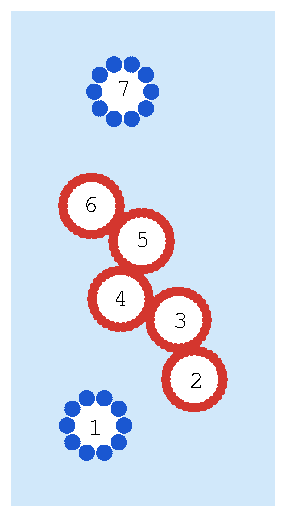
\includegraphics[scale=\marTwentySixSharedScale]{mar26_visualse_coarse_fine_fig2_demo.pdf}%
  }
  \hspace{1.5em}
  \subcaptionbox{}{%
    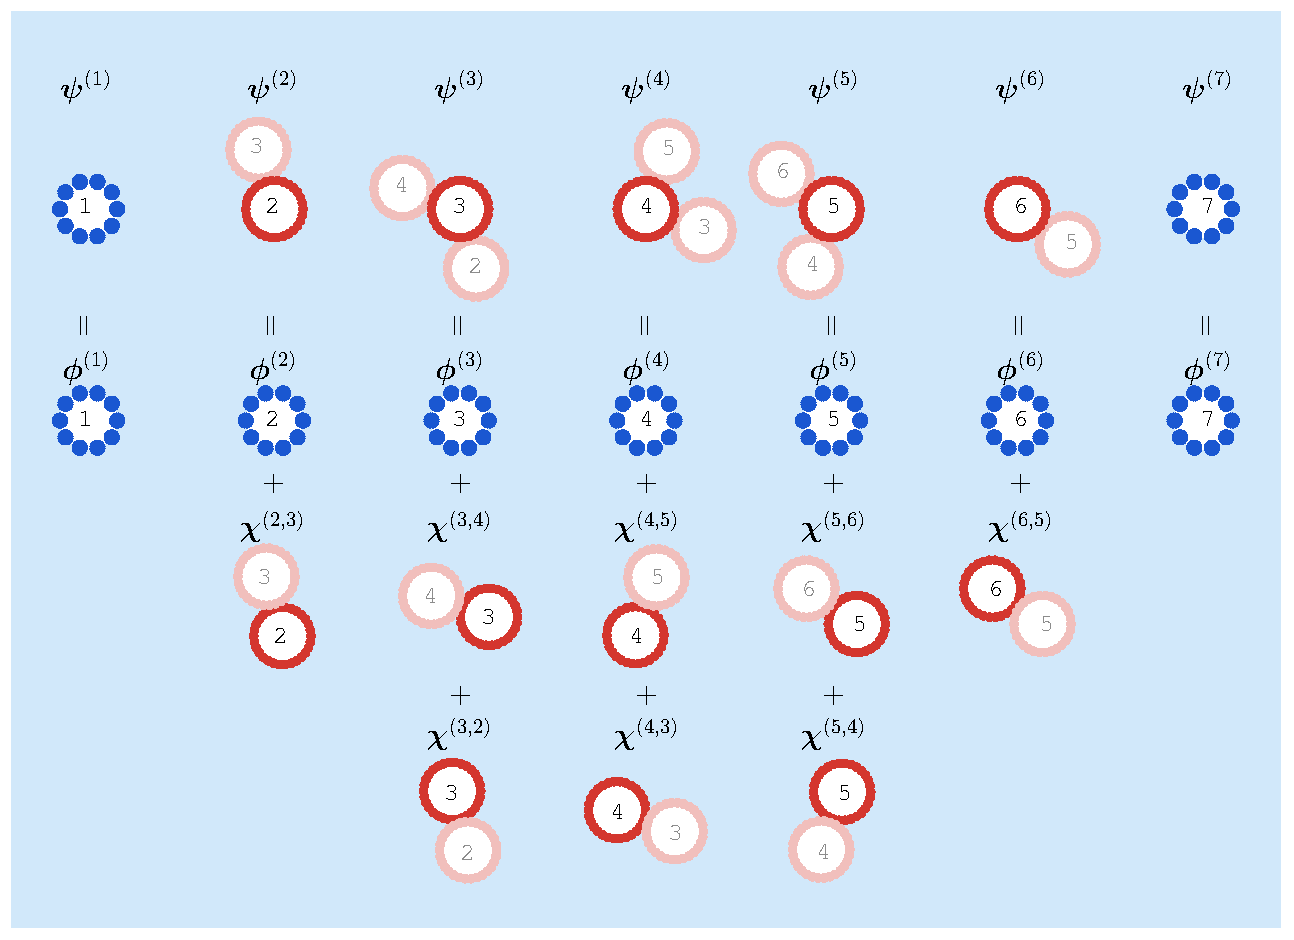
\includegraphics[scale=\marTwentySixSharedScale]{mar26_visualse_coarse_fine_fig3_demo.pdf}%
  }
  \caption{Coarse/fine visualisations shown at a common scale.}
\end{figure}

\end{document}
